\documentclass[a4paper,3p,sort&compress]{elsarticle}

\usepackage[draft]{hyperref}
\usepackage{url}
\usepackage{booktabs}
\usepackage{graphicx}
\usepackage{xspace} 
\usepackage{booktabs}
\usepackage{makecell}
\usepackage{lineno}
\usepackage{natbib}
\usepackage{amsmath}
\DeclareRobustCommand{\citeext}[1]{\citeauthor{#1}~\cite{#1}}

\usepackage[nomargin,inline,draft]{fixme}
\fxsetup{theme=color,mode=multiuser}
\FXRegisterAuthor{j}{jla}{\color{purple}JLA}
\FXRegisterAuthor{s}{spv}{\color{teal}SPV}
 
\journal{-}

%% `Elsevier LaTeX' style
\bibliographystyle{plain}
%%%%%%%%%%%%%%%%%%%%%%%

\begin{document}
\linenumbers

% Macro para escribir NO$_2$
\newcommand{\no}{NO\textsubscript{2}\xspace}

\begin{frontmatter}

  \title{Introducing a novel visualization technique for time series uncertainty visualization}


  \author{Sebasti\'an P\'erez Vasseur}
  \author{Jos\'e L. Aznarte}
  \address{Artificial Intelligence Department\\Universidad Nacional de
    Educaci\'on a Distancia --- UNED\\c/ Juan del Rosal, 16, Madrid, Spain}
  \ead{jlaznarte@dia.uned.es}
  

\begin{abstract}
  
\end{abstract}

\begin{keyword}
probabilistic forecasting \sep visualization \sep natural frequency chart
\end{keyword}

\end{frontmatter}

%\linenumbers

\section{Introduction}
\label{sec:intro}

During all the stages of data analysis, users are confronted with uncertainty, which can have 
several causes such as missing information, statistical errors or modelling approximations.
This uncertainty also affects forecasting models whose estimations are naturally 
subject to some degree of uncertainty as happens to any other model. One way to present this 
uncertainty is to provide a full probability distribution as an estimation instead of a single value. 
Probabilistic time series forecasting models are an example of this and they provide the full probability 
distribution of the future values of a time series.

As stated by Padilla et al. \cite{padilla_uncertainty_2021}, it is beneficial to take into account uncertainty when making decisions as it
helps to estimate the potential risks and rewards derived from decisions. For example, Pinson mentioned how uncertainty 
in wind energy forecasts optimized the use of this ressource. In air quality forecasting, we showed 
how probabilistic forecasting enables the estimation of the risk the No2 pollutant will surpass a certain threshold 
and become a danger to the city inhabitants. Rouston et al. \cite{roulston_laboratory_2006} indicated how analysts 
improved their rewards thanks to uncertainty when taking decisions from temperature forecasts.
Also, people already think in terms of uncertainty and they naturally expect it in the forecasts: 
for example, for weather forecast 
they already think in terms of temperature ranges or words which cover a range ("warm" or "cold"). As stated by Joslyn et al.
\cite{joslyn_communicating_2010} , 
those forecasts with uncertainty can validate or correct the invalid biases from their original expectations: Indeed,
it's easier to correct a range of values with another range of values rather than a single value.

However, there is a concern that people will not be able to understand predictions that come with uncertainty.
This fear is reinforced by cases where uncertainty seems to confuse the users. For example,
Belia et al \cite{belia_researchers_2005} showed that even leading researchers had 
trouble reading error bars. 
As Padilla et al. \cite{padilla_uncertainty_2021} 
points out, this could be due to to the abstract nature of the probability concepts or to poor communication techniques. 

One way to improve the communication of uncertainty is based on data visualization. Indeed, as 
stated by Islam et al. \cite{islam_overview_2019}, visualizations are easier for the human brain to understand and process.
For instance, Perez Cota et al. \cite{cota_importance_2014} mentions how visualization are playing an important role in the business 
environment where all the analytical tools are embracing visualization to better understand large quantities of data. 

As pointed out by Weiskopf et al. \cite{weiskopf_uncertainty_2022} or Padilla et al. \cite{padilla_uncertainty_2021}, 
there's existing research around uncertainty visualization 
but as pointed out by Leffrang et al. \cite{leffrang_should_2021} there's few research on uncertainty on time series forecasting. Also, 
estimating probabilities from the forecasts with uncertainty helps to estimate the risks and rewards derived from those 
decision. Therefore, we can ask ourselves how good are the different solutions derived from research in that area. 

Following this thought, we will present in section 2 the current research on uncertainty visualization. We will then
design different soutions applied to the Probabilistic time series forecasting models in section 3 and in section 4 and 5,
we will compare those methods against the question: how well can we estimate probabilities with it. 
For that, inspired by Brennen et al. \cite{brennen_instrument_2018}, we propose a social experiment where we will compare different charts 
in terms of probability reading. 

We will use as an application ground for this comparison a probabilistic forecast of NO levels 
in the city of Madrid. This forecast contains the full predicted distribution of NO levels over time
and we display this very same time series with uncertainty in each of the visualization mentioned above. 
We then estimate for each one how well its numeric values are read by assessing how several individuals read 
and understand the charts.

\section{State of the art}
\label{sec:results}

As noted by Joslyn et al. \cite{joslyn_communicating_2010},the shortcomings in uncertainty visualization lead to a new surge of 
research in visualization techniques. 

Pang et al. \cite{pang_approaches_1997} were the first to gather uncertainty visualization techniques and classify them in 
order to bring order to the field and help 
practitioners choose the right visualization. However, their taxonomy did not explain how the visualization works nor helped creating new 
ones. Following uncertainty visualization surveys were based on data types (Potter et al. \cite{potter_quantification_2012} and Brodlie et al. 
\cite{brodlie_review_2012}), 
sources of uncertainty (Bonneau et al. \cite{bonneau_overview_2014}), types of uncertainty 
(Ristovski et al. \cite{ristovski_uncertainty_2014}). Jena et al. \cite{jena_uncertainty_2020} classified the techniques 
based on the publication channel and audience and even made their findings available online as a 
public web site. 

The most notable work is the classifications delivered by Padilla et al. \cite{padilla_uncertainty_2021} which classifies according to 
the type of visual mapping. They provide the main types of uncertainty visualization techniques with their shortcomings and 
explain to the reader that there's no one size-fits-all solution and that visualization technique must be chosen according to their use case.

According to them, one of the most typical approaches, Visual Boundaries such as isocontours and error 
bars display value areas within a certain confidence interval. The problem with this approach is 
that individuals may exclude as possible, values outside the confidence interval, which are still 
possible, only less probable. Also, as stated previously, Belia et al \cite{belia_researchers_2005} showed that even leading researchers had 
trouble reading error bars as they confused 
standard errors and confidence intervals. In addition, Joslyn and LeClerc showed that individuals could also be inclined to take uncertain 
information as deterministic, for example by considering the confidence interval for whether temperature 
forecast as high and low temperature. 

As stated by Padilla et al. \cite{padilla_uncertainty_2021}, one possible solution to this problem is the use of HOPs 
(hypothetical outcome plot). HOPs display 
sequentially in an animation, random values from a distribution. However, this technique can not be 
applied to static visualizations and requires media formats like video or animated images: This makes difficult the distribution 
of that type of visualization.

An alternative approach, Visual Semiotics uses visual encoding such as fuzziness or color to represent 
the probability of a certain value. An example of this would be the use of gradients to represent the 
full probabiliity distribution. Neverthless, this type of encoding makes it difficult to read specific 
values. 

Finally, Frequency Framing uses natural frequencies to display probabilities. As noted by Gerd 
Gigerenzer, individuals prefer frequencies or ratio, like 1/10, when understanding probability. This has 
lead to the development of the quantile dot plot. This plot, created by Kay et al. \cite{2016-when-ish-is-my-bus}
\cite{2016-when-ish-is-my-bus} 
represents 
the probability distribution with dots: by using 20 dots, each would represent 1/20 probability 
and are placed according 
to the quantiles of the distribution. Quantile dot plot have proved to lead to better distribution 
understanding and probability estimates reading. 

However those approaches do not address specifically the problem of uncertainty in the case of time series.
The visualizations would need to show the evolution of uncertainty in time: this 
is especially challenging as a visualization must display several distributions in a constrained space.  
As pointed out by Leffrang et al. \cite{leffrang_should_2021}, not much research has been applied to this 
field. 
However, we can apply for this problem some of the solutions described above such as confidence interval charts or 
box plots (visual boundaries) or gradient charts (visual semiotics). However, we have not seen yet a solution involving 
frequency framing. 

Once all this visualizations are defined, we should find a way to compare them. It it true that as stated by van Wijk,
data visualization can be considered an art and therefore subject to criteria like taste or design aesthetics.

However, as noted by Pang et al. \cite{pang_approaches_1997}, the basic methodology to compare visualizations is to measure how accurate is the 
decoding of the visualization: we compare the value encoded in the visualization with the value read
by the user. In their classical paper, Cleveland et al. \cite{cleveland_graphical_1984} produced a ranking of visual encodings for numerical values 
with position being the most accurate encoder. However, as noted by Brennen et al. \cite{brennen_instrument_2018}
the complexity of a visualization could lead to better readability but higher time to read the chart. Also, 
they noticed that those measures do not take into account the perception of the user, specially when the visualization
is showing uncertainty. Therefore they developed a methodology 
to systematically evaluate the performance of uncertainty visualizations, based on four measures: 
cognitive load, confidence, reading error and time to read. 

\section{Time Series probabilistic charts}  
\label{sec:time_series}

Based on the research above, we have identified the following charts as suitable to display 
uncertainty in time series.

The first one is the confidence interval chart  which shows in a line the evolution of the 
median of the distribution
 over time alongside 2 lines: the evolution of the 5\% and 95\% percentile of the distribution. 
 User estimates the probabilities with the distance of the points to those lines.

The box plot chart shows different percentile with “boxes”. For each point in time, a white 
line shows the location of mean, then 2 boxes display different percentiles: the
first rectangle (or box) lower and upper part are located 
at the 25\% and 75\% percentile respectively, a narrower box upper and lower part shows 
the 5\% and 95\% percentile and finally a line’s edge shows the 1\% and 99\% percentile. 
This visual boundary representation shows more percentile than the confidence interval and 
is recommended when the distribution is not symmetrical and to show the edges of the distribution.

The gradient chart shows the evolution of the median in a line and then displays the different percentiles
with overlapping areas whose color corresponds to the percentile. We end up having an area with a gradient 
delimited by 2 lines: the 1\% and 99\% percentile. This representation allows to have the
 full range of percentiles represented.

The 3 methods described above have been used in the literature as a way to display the overall uncertainty 
of the target variable. However, they are not designed for probability readability: for example, to determine 
the probability the target variable is within a certain range or above a certain value. Also,
each of the methods have their own shortcomings. The confidence interval gives a false sense of determinism as mentioned previously
and values outside of the interval will not be taken into account. The confidence interval is also not a good solution 
when the distribution of the target variable has a long tail. The box plot shows only some percentiles and it can be difficult to 
estimate the probabilities from the boxes boundaries. Finally, although the gradient displays the most information, it has been 
proven that color is not 
a good visual encoding and is more difficult to read than other encodings. We plan on showing those shortcomings during the comparison in our experiments.

Since no solution was based on natural frequencies, we decided to apply the idea for time series and design the natural frequency time chart.
This visualization is a novel technique based on frequency framing and has 
specifically been designed for probability readability. First, 
it shows the evolution of the median of the distribution in a line. And then, for each time 
step, 10 percentiles from 5\% to 95\% (5\%, 10\%, 15\%, ...) are represented: this way, we can estimate the percentage 
probability of being in an interval as 10 times the number of circles in that interval. 
We have chosen 10 percentiles as it makes it easy to calculate the probability (just multiply by 10), also a higher number
would have cramped the chart and made it difficult to view the circles as separate. 

Figure \ref{figure:charts} shows a summary of the described probabilistic time series charts.

\begin{figure}
  \centering
  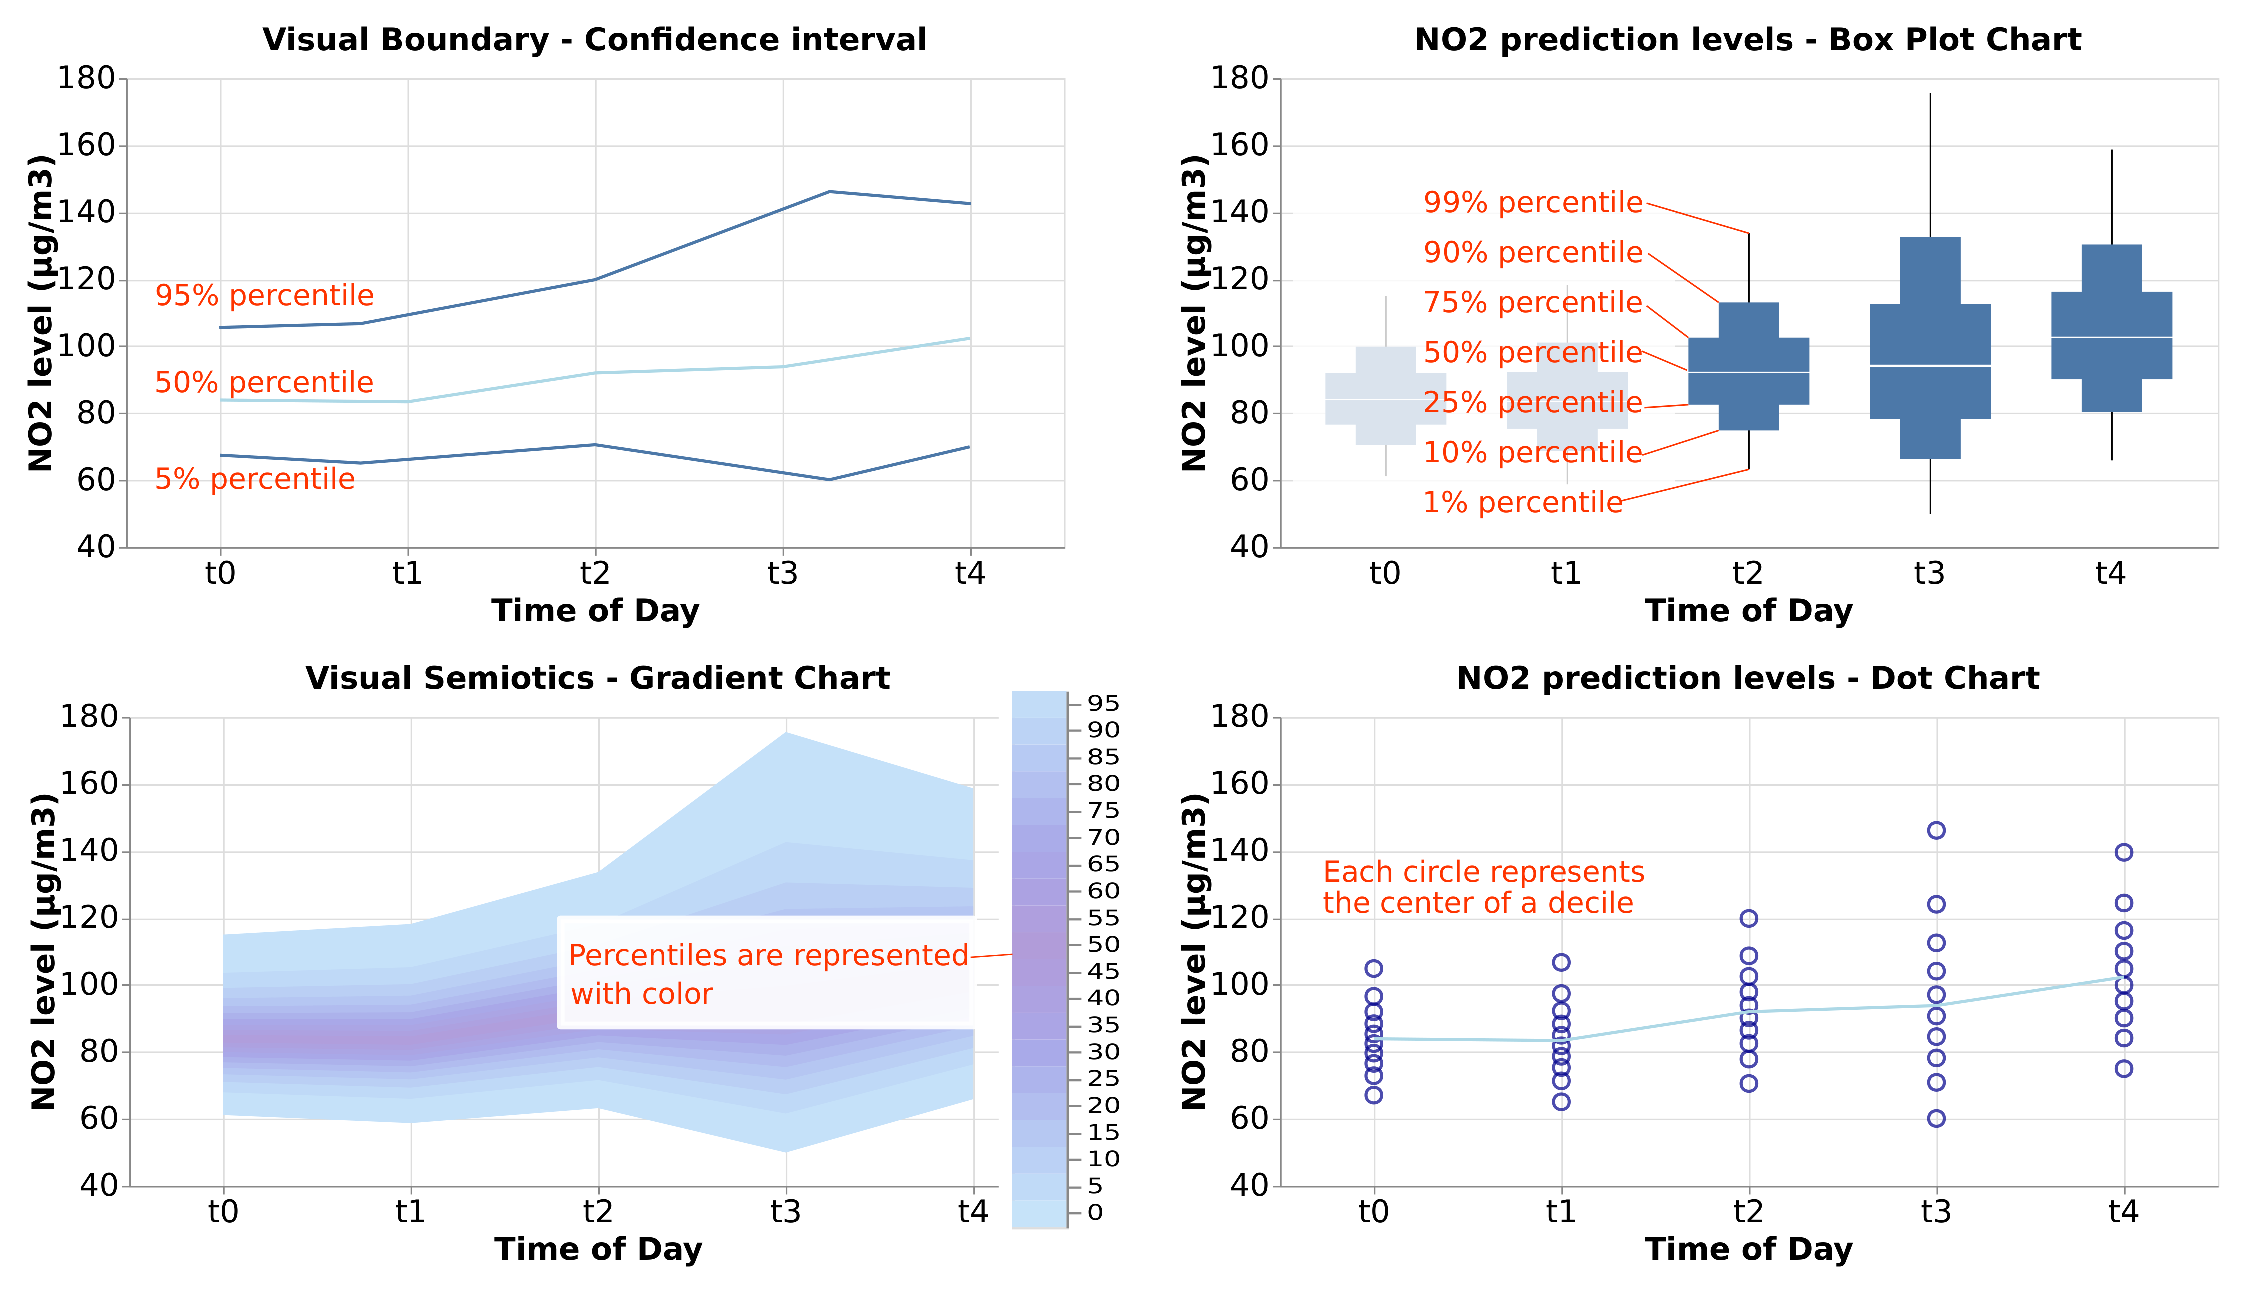
\includegraphics[width=.9\textwidth]{charts_vector} 
  \caption{\label{figure:charts} Probabilistic Forecast of NO2 levels in Madrid with different types of time Series Chart. 
  Top Left: Confidence Interval. Top Right: Box Plot. 
  Bottom Left: Gradient Chart. Bottom Right: Natural Frequency Time Chart. }
\end{figure} 

\section{Experimental Design}
\label{sec:exp_design}

We would like to compare the charts described in the previous section (displayed in Figure 1) 
in terms of probability 
reading, ie how well 
can the charts communicate the probability that the evolving target is within a certain interval 
at a certain time point.
 For this, we will use as inspiration the experiments of Brennen et al. \cite{brennen_instrument_2018}
and will use similar metrics 
as them: readinig error, time to answer, cognitive load and perception. The reading error will be estimated as the 
absolute value of the difference between the read probability and the real probability. The time to answer 
will be calculated from the moment the reader sees the chart until he submits his answer. The cognitive 
load and the confidence are the perceived difficulty reading the charts and the perceived confidence on 
the accuracy of 
the answer. Both of those metrics are requested explicitly to the reader.

We have built a probabilistic time series forecasting model that estimates the distribution of NO 
levels in one of the air quality stations in Madrid. Those stations measure the level of certain 
pollutants like O3 or NO and serve as a monitoring tool for the air quality of the city. If the pollutant 
reach certain levels, it can be dangerous for the city inhabitants. Therefore it becomes necessary 
for the city administration to 
forecast the air quality levels to take decisions based on it (like limiting car traffic to reduce it beforehand).
Our model produces an hourly forecast for the next day of one of the pollutants: NO. This forecast contains
for each hour of the day the probability distribution of the target variable and therefore provides the evolution 
of the probability distribution of the target variable (NO level).

We will display this very same evolution on each of the 4 charts and we will evaluate how well users can 
read the probability the NO level is within a certain range at a certain hour. 

For this, we request the participation of users through the Amazon Mechanical Turk website. 
This service picks randomly 100 individuals with a minimum skill set (as proposed by Brennen 
et al. \cite{brennen_instrument_2018}, we select Master level participants, who are workers who 
''have consistently demonstrated a high degree of success in performing a wide range of HITs across a 
large number of Requesters'').

We then implemented a web site which guides the user through a presentation of the chart and the questions.
Indeed,  each individual is presented a unique type of chart from the 4 presented above, gets a brief 
explanation on how it works and they are asked to estimate 5 probabilities at 5 different moments from the chart. 
An example question is: 
"What is the probability of the NO2 levels being between 150 and 200 on 
November 21st at 22:00 ?". The 5 questions were:
\begin{itemize}
  \item What is the probability of the NO2 levels being between 150 and 200 on November 21st at 22:00 ?
  \item What is the probability of the NO2 levels being between 70 and 120 on November 21st at 14:00 ?
  \item What is the probability of the NO2 levels being above 150 on November 22nd at 09:00 ?
  \item What is the probability of the NO2 levels being between 50 and 100 on November 21st at 11:00 ?
  \item What is the probability of the NO2 levels being above 200 on November 21st at 20:00 ?
\end{itemize}

For each question, we are measuring the accuracy and the time it took to 
perform each estimation. Once the individuals have estimated the probabilities, they are asked how confident they 
felt and how difficult the task was considered.

We are testing 80 individuals: 20 individuals per type of chart and therefore we have 100 answers per 
type of chart.

\section{Results}
\label{sec:results}


After gathering all the answers from the participants, we calculated the different metrics described in the previous section and 
then built figure \ref{figure:errors} 
which displays 
the distribution of the reading error, the confidence and the perceived difficulty per type of chart. 

It is interesting to note that although we selected users with master level, we did receive off-topic answers with probabilities 
above 1 or a probability as an interval. This could be due a lack of statistical knowledge from those 
users and reinforces the fears discussed in the introduction. We identified 9 users from 80 whose answers could not be used because of those reasons.

In the reading errors chart of figure \ref{figure:errors}, the worst chart in terms of readability seems to be the 
gradient chart and the best is the natural frequency time chart as it has a much lower reading error than the other charts. As stated before, 
gradient charts are designed to showcase a general overview of the distribution as they represent the evolution of the
full range of percentiles, however as shown by Cleveland et al., the "color" visual encoding is one of the 
worst encoders and limits the readability of the chart. Box plots and confidence interval have similar reading errors: This is surprising
as box plots display more percentiles than the confidence interval. On the other hand, natural 
frequency charts have a much lower readability error and we can see how the use of natural frequencies creates a more accurate reading experience.

Confidence and perceived difficulty charts (also shown on figure \ref{figure:errors}) mirror the results in the reading error chart.
It also shows the superior ease of use 
of the natural frequency time chart: Users reported higher levels of confidence and 
lower levels of perceived difficulty for this chart. Also, although box plot and confidence interval have similar reading errors,
user perceive the confidence interval as more difficult to read and are less confident with their readings. This can be explained with 
the simpler nature of the confidence interval which only displays 2 percentiles and demand users to estimate the position of the other 
percentiles only from those 2.

We can perform a statistical comparison of the reading errors of each chart with the Krustal-wallis test \cite{krustal} and 
the Quade test \cite{quade_rank_1967}. Both tests have a 
significantly low p-value (6.6e-10 and 5.6e-07) and confirms our conclusions from the visual inspection of the chart.

Figure \ref{table:resultsperquestion} shows the error per question and interestingly we can see that the open interval questions (questions 3 and 5) 
had less errors than the other questions. Question 4 error rate is high as the distribution of the target at that time was concentrated in a relatively 
small interval and it was more difficult to estimate the probability in that area. 

\begin{figure}
  \centering
  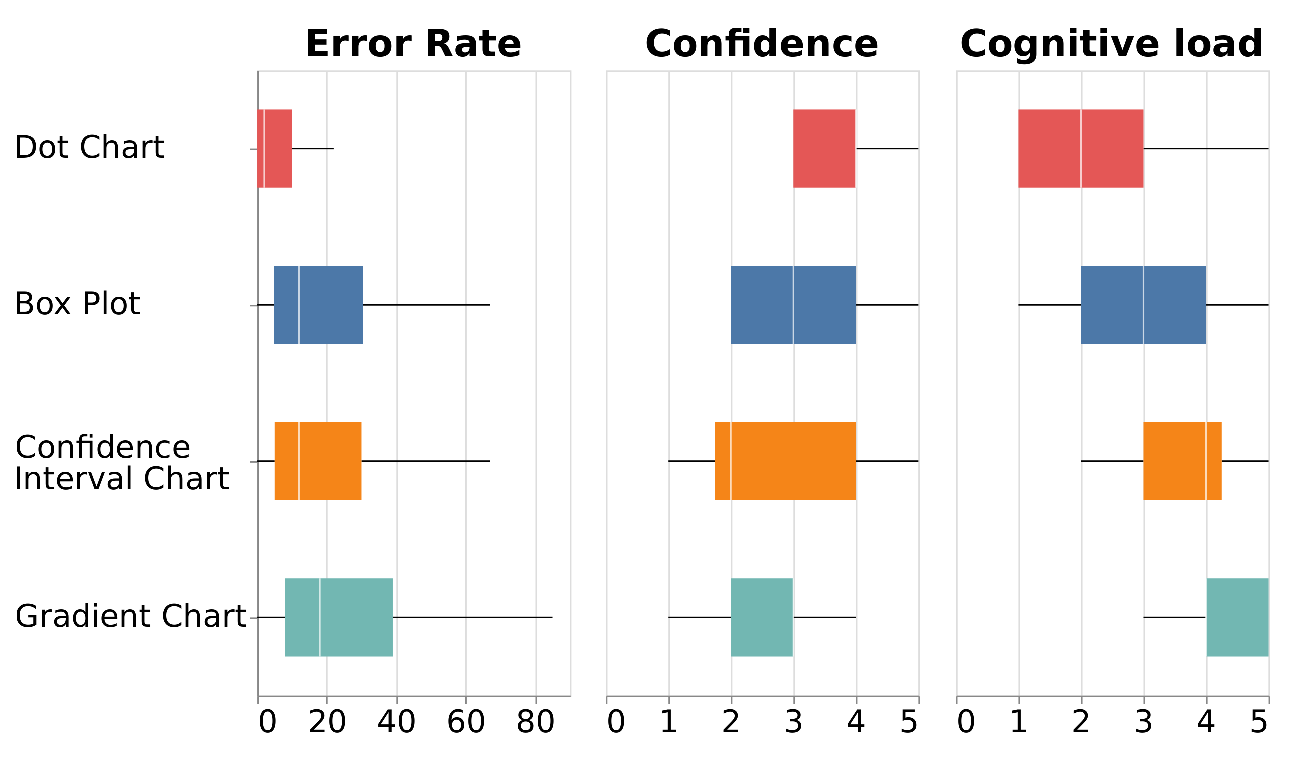
\includegraphics[width=0.8\textwidth]{comparison}
  \caption{\label{figure:errors}Reading Error, confidence and perceived difficulty per 
  type of visualization. Black vertical line represents median.
  The whiskers represent the 10 and 90 percentile and the box shows the 25 and 
  75 percentile.}
\end{figure}


\begin{table}[h!]
  \centering
  \begin{tabular}{lrr}
    \toprule
    {}Question &     Error Mean &        Error Std Deviation \\
    \midrule
    1 &  19.4 &  16.8 \\
    2 &  20.7 &  12.1 \\
    3 &  10.9 &  18.9 \\
    4 &  27.0 &  26.9 \\
    5 &  16.1 &  15.6 \\
    \bottomrule
    \end{tabular}
  \caption{Error}
  \label{table:resultsperquestion}
  \end{table}

\begin{figure}
  \centering
   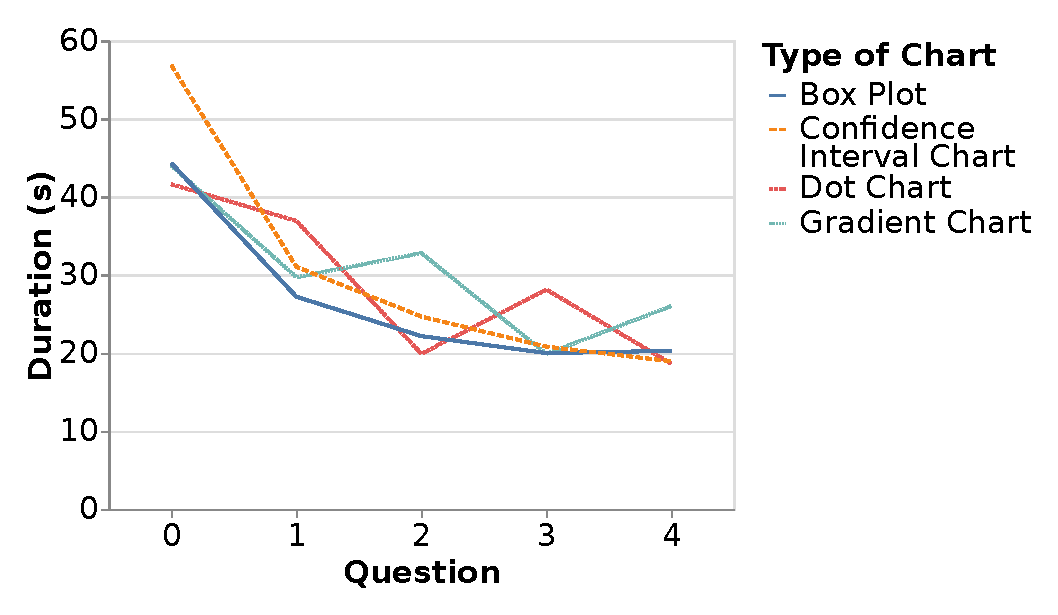
\includegraphics[width=0.6\textwidth]{duration_evo2}
  \caption{\label{figure:duration} Median Time it took to answer each question for each of the types of chart.}
\end{figure}  

We also recorded the time it takes to answer each of the questions and built the chart in figure \ref{figure:duration}. We 
can see that the answering times are similar for every chart and that this time decreases as the users answer questions.
This must be due to the fact that they are learning to use the charts and needing less time to answer the questions.
However, due to the higher perceived difficulty, we were expecting different answering times. Perhaps if we had 
increased the number of questions, we would have seen a difference in the answering time (or users quitting the test before 
its end).


\section{Conclusions}
\label{sec:concl}

Although we could remark that the gradient chart, the box plot or the confidence interval charts are very good at 
providing an overall picture of the uncertainty in the time series, we can see from this work that the application of natural 
frequencies in an uncertainty chart does indeed
provide better numeric readability than any previous alternative. Natural frequencies does indeed simplify 
the statistic knowledge requirement and is also easier to read as it consists on counting.
We could improve even more the ease of use with interactive elements in the chart: for example
by applying different colors to the circles within a certain interval defined by the user interactively.
An interactive chart with zoom capabilities would have solved that 
issue in question 4.

This type of chart is less well known that the other alternatives and an information effort should be made to motivate 
researchers and the general public to use it.

\section{References}
\label{sec:ref}


\bibliography{refs}

\end{document} 

